\chapter{Un premier regard sur les cellules}\label{ch:g5:first-look-at-cells}

Regarde le dos de ta main~: une \omterm{def:g1:the-five-senses:sense}{peau} lisse, une surface d'un seul
tenant. Imagine maintenant une loupe assez puissante pour grossir
mille fois. La surface lisse se dissoudrait en un pavage de
minuscules compartiments, ajustés les uns aux autres comme des
dalles --- et tous les \omterm{def:g1:living-or-not:living}{êtres vivants} que tu as croisés dans ce
livre, de la mousse à la baleine, sont pavés de la même façon. Le
plus grand secret de la \omterm{def:g1:living-or-not:living}{biologie} est petit.

\section{Les êtres vivants sont faits de cellules}

\begin{definition}[Cellule]\label{def:g5:first-look-at-cells:cell}
Une \emph{cellule}\index{cellule} est la plus petite brique vivante
d'un \omterm{def:g1:living-or-not:living}{être vivant}. Presque toutes les cellules sont bien trop petites
pour être vues à l'\omterm{def:g1:the-five-senses:sense}{œil} nu~; un corps est bâti de cellules comme un
mur est bâti de briques. Ton propre corps est fait de dizaines de
milliers de milliards de cellules.
\end{definition}

\begin{proposition}[Le principe cellulaire]\label{prop:g5:first-look-at-cells:principle}
Tout \omterm{def:g1:living-or-not:living}{être vivant} est fait de \omterm{def:g5:first-look-at-cells:cell}{cellules} --- chaque \omterm{def:g1:animals-around-us:animal}{animal}, chaque
\omterm{def:g1:plants-around-us:plant}{plante}, chaque champignon, jusqu'aux \omterm{def:g1:living-or-not:living}{êtres vivants} qui n'ont
qu'\emph{une} \omterm{def:g5:first-look-at-cells:cell}{cellule}. Cette construction partagée est l'un des
grands signes de l'\emph{unité du vivant}\index{unité du vivant}~:
si différentes que soient la pâquerette et la baleine, de près elles
sont bâties du même genre de petites unités vivantes.
\end{proposition}
\admitted

\begin{example}[Petit comment~?]\label{ex:g5:first-look-at-cells:small}
Une \omterm{def:g5:first-look-at-cells:cell}{cellule} courante de ton corps mesure environ un cinquantième de
millimètre. Aligne-en $50$ et elles couvrent un millimètre --- un
point de crayon suffirait à cacher le défilé. Voilà pourquoi
personne n'a soupçonné les \omterm{def:g5:first-look-at-cells:cell}{cellules} pendant presque toute
l'histoire humaine~: les briques du vivant sont plus petites que la
plus petite tache visible à l'\omterm{def:g1:the-five-senses:sense}{œil}.
\end{example}

\section{L'instrument qui les a révélées}

\begin{definition}[Microscope]\label{def:g5:first-look-at-cells:microscope}
Un \emph{microscope}\index{microscope} est un instrument dont les
lentilles grossissent des centaines de fois les très petites choses.
Braqué sur de fines tranches de matière vivante, il a révélé ce
qu'aucun \omterm{def:g1:the-five-senses:sense}{œil} n'avait jamais vu~: les \omterm{def:g5:first-look-at-cells:cell}{cellules}. Le nom lui-même vient
d'un premier observateur qui trouva que les petits compartiments
d'une tranche de liège ressemblaient aux petites chambres des moines
--- des \emph{\omterm{def:g5:first-look-at-cells:cell}{cellules}}.
\end{definition}

\begin{omfigure}
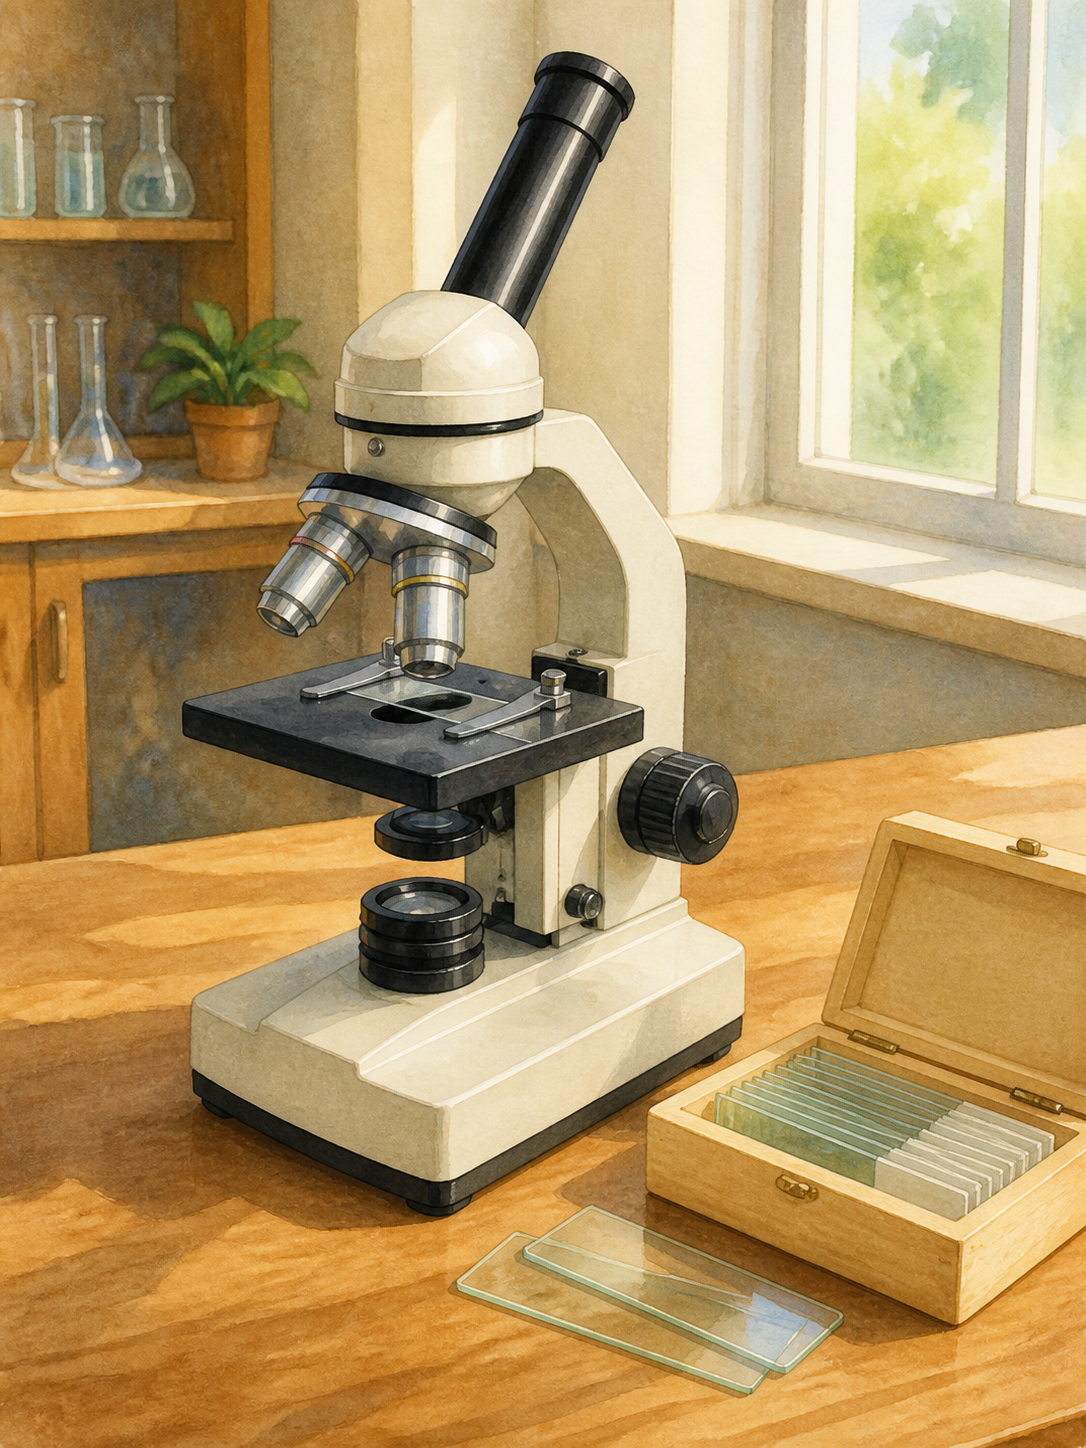
\includegraphics[width=0.44\linewidth]{images/book1/ai/g5-cells-microscope.png}

{\small L'instrument qui a révélé les \omterm{def:g5:first-look-at-cells:cell}{cellules}~: des lentilles, de
la lumière, et une fine tranche sur une lame de verre.}
\end{omfigure}

\begin{example}[Deux classiques sous l'objectif]\label{ex:g5:first-look-at-cells:classics}
Deux observations que tout \omterm{def:g5:first-look-at-cells:microscope}{microscope} d'école peut refaire~: un
lambeau de la fine pellicule intérieure d'un oignon montre de nettes
rangées de \omterm{def:g5:first-look-at-cells:cell}{cellules} en forme de briques, paroi contre paroi~; un
léger grattage de l'intérieur de la joue montre des \omterm{def:g5:first-look-at-cells:cell}{cellules}
dispersées et plus rondes --- les tiennes. Végétal et \omterm{def:g1:animals-around-us:animal}{animal}, \omterm{def:g3:bones-and-muscles:skeleton}{côte} à
\omterm{def:g3:bones-and-muscles:skeleton}{côte}, tous deux cellulaires.
\end{example}

\begin{omfigure}
\begin{minipage}[t]{0.48\linewidth}\centering
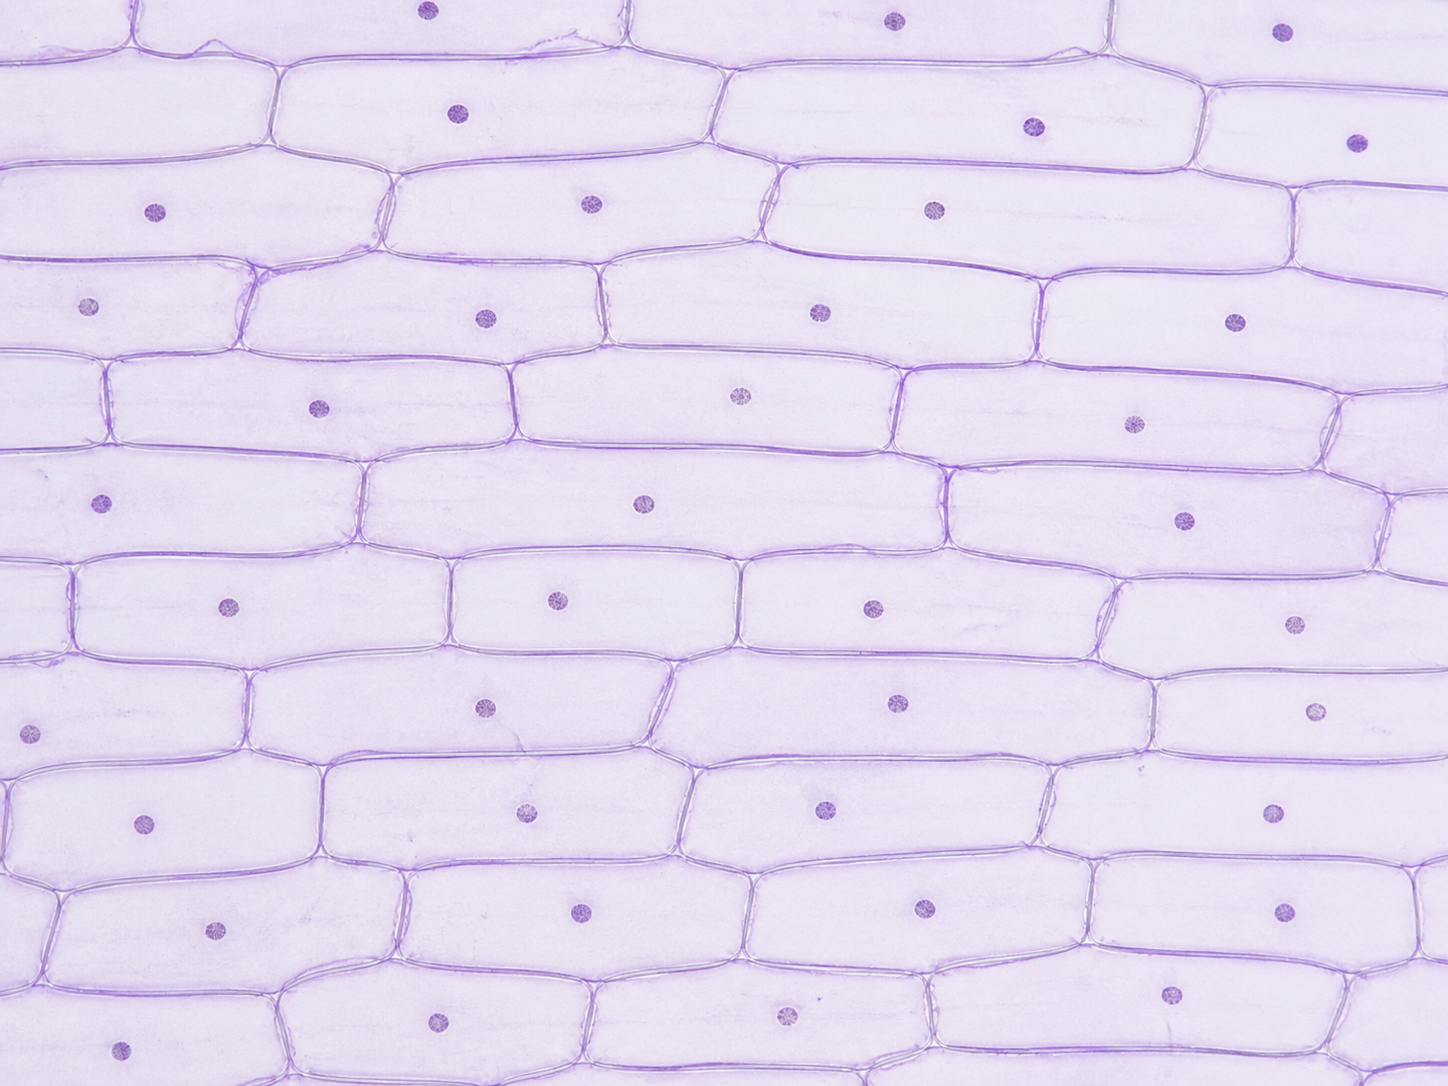
\includegraphics[width=\linewidth]{images/book1/ai/fig-onion-cells.png}

{\small pellicule d'oignon~: des \omterm{def:g5:first-look-at-cells:cell}{cellules}\\ en briques bien rangées}
\end{minipage}\hfill
\begin{minipage}[t]{0.48\linewidth}\centering
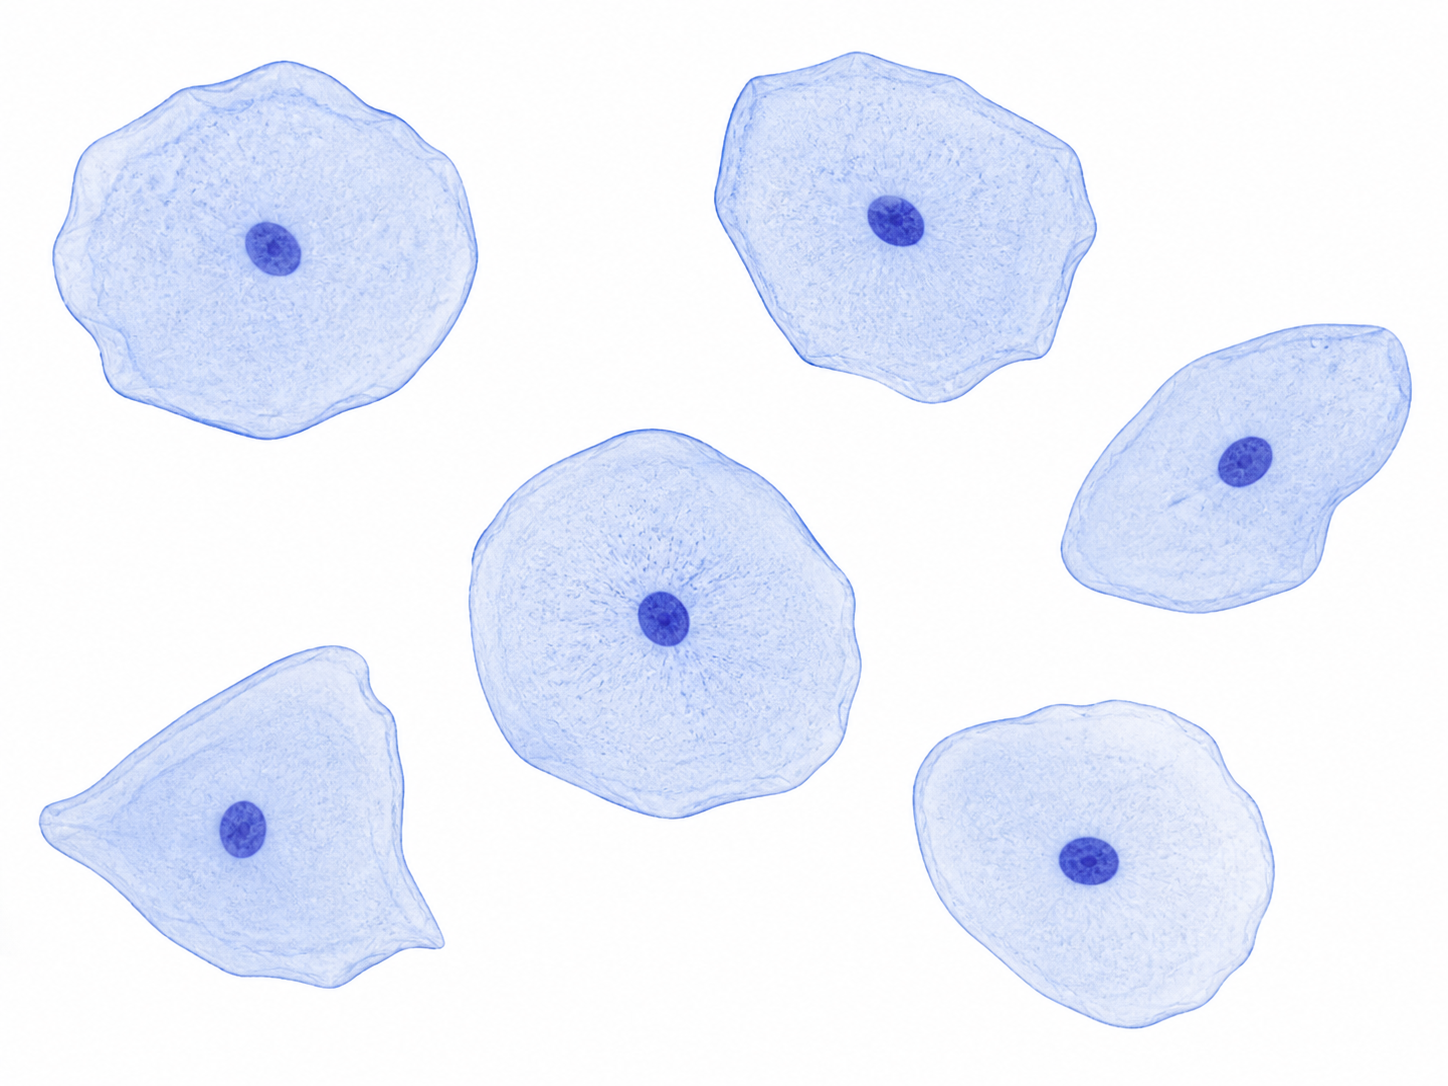
\includegraphics[width=\linewidth]{images/book1/ai/fig-cheek-cells.png}

{\small grattage de joue~: des \omterm{def:g5:first-look-at-cells:cell}{cellules}\\ plus rondes, dispersées}
\end{minipage}

\medskip
{\small Au \omterm{def:g5:first-look-at-cells:microscope}{microscope}~: des \omterm{def:g5:first-look-at-cells:cell}{cellules} d'oignon et des \omterm{def:g5:first-look-at-cells:cell}{cellules} de
joue. Chaque compartiment --- avec sa petite tache sombre --- est
une \omterm{def:g5:first-look-at-cells:cell}{cellule}.}
\end{omfigure}

\begin{remark}[La tache sombre]\label{rem:g5:first-look-at-cells:nucleus}
Dans les deux vues, la plupart des \omterm{def:g5:first-look-at-cells:cell}{cellules} montrent à l'intérieur
une petite tache plus sombre~: le centre de commande de la \omterm{def:g5:first-look-at-cells:cell}{cellule},
appelé son \emph{noyau}\index{noyau}. Ce avec quoi le noyau
commande --- le fameux fil d'instructions enroulé dedans --- est une
histoire pour les années ultérieures de ce livre~; pour l'instant,
retiens seulement que les petites chambres ne sont pas vides.
\end{remark}

\section{D'une cellule à un corps}

\begin{proposition}[Les corps grandissent par leurs cellules]\label{prop:g5:first-look-at-cells:growth}
Un corps grandit, et se répare, parce que ses \omterm{def:g5:first-look-at-cells:cell}{cellules} savent se
\emph{diviser}~: une \omterm{def:g5:first-look-at-cells:cell}{cellule} se partage en deux \omterm{def:g5:first-look-at-cells:cell}{cellules} vivantes,
deux en quatre, et ainsi de suite. Grandir en taille
(\cref{prop:g3:stages-of-life:animals}) est, en dessous, une
multiplication de \omterm{def:g5:first-look-at-cells:cell}{cellules}~; une éraflure qui guérit
(\cref{rem:g3:bones-and-muscles:alive}) est une reconstruction par
les \omterm{def:g5:first-look-at-cells:cell}{cellules}. Et tout corps, même le plus grand, a commencé par une
\emph{seule \omterm{def:g5:first-look-at-cells:cell}{cellule}} --- la \omterm{def:g4:animal-reproduction:sexual}{cellule œuf} fécondée de
\cref{def:g4:animal-reproduction:sexual}.
\end{proposition}
\admitted

\begin{example}[D'une seule à des milliers de milliards]\label{ex:g5:first-look-at-cells:one}
La \omterm{def:g4:animal-reproduction:sexual}{cellule œuf} fécondée se divise en $2$ \omterm{def:g5:first-look-at-cells:cell}{cellules}, puis $4$, $8$,
$16$ \dots{} Répétée pendant des mois et des années, la division a
bâti les dizaines de milliers de milliards de \omterm{def:g5:first-look-at-cells:cell}{cellules} qui lisent
cette phrase. Chaque \omterm{def:g5:first-look-at-cells:cell}{cellule} de toi descend de cette première.
\end{example}

\begin{remark}[Des vies entières dans une cellule]\label{rem:g5:first-look-at-cells:onecelled}
Certains \omterm{def:g1:living-or-not:living}{êtres vivants} ne dépassent jamais une seule \omterm{def:g5:first-look-at-cells:cell}{cellule} --- et
n'ont besoin de rien de plus. Une goutte d'eau de mare en grouille~:
des \omterm{def:g5:first-look-at-cells:cell}{cellules} uniques qui nagent, se nourrissent et se divisent, des
vies entières à l'échelle du \omterm{def:g5:first-look-at-cells:microscope}{microscope}. Les \omterm{def:g1:healthy-habits:germs}{microbes} de
\cref{def:g1:healthy-habits:germs} sont surtout de tels \omterm{def:g1:living-or-not:living}{êtres
vivants} à une seule \omterm{def:g5:first-look-at-cells:cell}{cellule} --- de vieilles connaissances, munies
maintenant d'une explication.
\end{remark}

\section{Exercices}

\begin{exercise}[$\star$]\label{exo:g5:first-look-at-cells:1}
Qu'est-ce qu'une \omterm{def:g5:first-look-at-cells:cell}{cellule}~? Combien y en a-t-il à peu près dans ton
corps~?
\end{exercise}

\begin{exercise}[$\star$]\label{exo:g5:first-look-at-cells:2}
Pourquoi personne n'a-t-il connu les \omterm{def:g5:first-look-at-cells:cell}{cellules} pendant presque toute
l'histoire~? Quel instrument a changé cela~?
\end{exercise}

\begin{exercise}[$\star$]\label{exo:g5:first-look-at-cells:3}
Décris ce que le \omterm{def:g5:first-look-at-cells:microscope}{microscope} montre dans la pellicule d'oignon, et
dans un grattage de joue. Qu'ont en commun les deux vues~?
\end{exercise}

\begin{exercise}[$\star$]\label{exo:g5:first-look-at-cells:4}
Comment s'appelle la petite tache sombre visible dans la plupart des
\omterm{def:g5:first-look-at-cells:cell}{cellules}~?
\end{exercise}

\begin{exercise}[$\star$]\label{exo:g5:first-look-at-cells:5}
Combien de \omterm{def:g5:first-look-at-cells:cell}{cellules} du corps, alignées, couvrent un millimètre ---
et quelle est la longueur d'une \omterm{def:g5:first-look-at-cells:cell}{cellule}, en millimètres~?
\end{exercise}

\begin{exercise}[$\star$]\label{exo:g5:first-look-at-cells:6}
Que font les \omterm{def:g5:first-look-at-cells:cell}{cellules}, en dessous, quand un enfant grandit~? Et
quand un \omterm{def:g1:my-body:joint}{genou} éraflé guérit~?
\end{exercise}

\begin{exercise}[$\star$]\label{exo:g5:first-look-at-cells:7}
Par combien de \omterm{def:g5:first-look-at-cells:cell}{cellules} tout corps humain a-t-il commencé~? Quelle
était cette première \omterm{def:g5:first-look-at-cells:cell}{cellule}, d'après
\cref{def:g4:animal-reproduction:sexual}~?
\end{exercise}

\begin{exercise}[$\star$]\label{exo:g5:first-look-at-cells:8}
Une \omterm{def:g5:first-look-at-cells:cell}{cellule} se divise en $2$~; chacune de celles-là se divise à son
tour, et ainsi de suite. Poursuis le doublement à partir de $1$~:
combien de \omterm{def:g5:first-look-at-cells:cell}{cellules} après $5$ divisions~? Après $10$~?
\end{exercise}

\begin{exercise}[$\star\star$]\label{exo:g5:first-look-at-cells:9}
Explique la phrase~: «~la pâquerette et la baleine montrent l'\omterm{prop:g5:first-look-at-cells:principle}{unité
du vivant}~». Que partagent-elles, d'après
\cref{prop:g5:first-look-at-cells:principle}~?
\end{exercise}

\begin{exercise}[$\star\star$]\label{exo:g5:first-look-at-cells:10}
Une goutte d'eau de mare contient des \omterm{def:g1:living-or-not:living}{êtres vivants} d'une seule
\omterm{def:g5:first-look-at-cells:cell}{cellule} chacun. Confronte-les aux signes de la vie de
\cref{prop:g1:living-or-not:signs}~: quels signes une seule \omterm{def:g5:first-look-at-cells:cell}{cellule}
peut-elle montrer~?
\end{exercise}

\begin{exercise}[$\star\star\star$]\label{exo:g5:first-look-at-cells:11}
Les \omterm{def:g5:first-look-at-cells:cell}{cellules} d'un éléphant ont à peu près la même taille que celles
d'une souris. Qu'est-ce qui rend alors l'éléphant plus grand --- des
\omterm{def:g5:first-look-at-cells:cell}{cellules} plus grandes, ou davantage de \omterm{def:g5:first-look-at-cells:cell}{cellules}~? Que dit ta réponse
sur la façon dont on grandit, d'après
\cref{prop:g5:first-look-at-cells:growth}~?
\end{exercise}
